\documentclass[12pt,a4paper]{ctexart}

\usepackage{booktabs}
\usepackage{tabularx}
\usepackage{longtable}
\usepackage{amsmath}
\usepackage{array}

% 页面设置
\usepackage{geometry}
\geometry{left=2.5cm,right=2.5cm,top=2.5cm,bottom=2.5cm}

% 字体与行距
\setCJKmainfont{Noto Serif CJK SC}
\setmainfont{Times New Roman} % 英文正文 Times New Roman
\linespread{1.5}
\setlength{\parindent}{2em}
\setlength{\parskip}{0pt}

% 列表格式
\usepackage{enumitem}
\setlist[itemize]{noitemsep, topsep=2pt}
\setlist[enumerate]{noitemsep, topsep=2pt}

% 图形
\usepackage{graphicx}
\usepackage{float}
\usepackage{tikz}
\usetikzlibrary{arrows.meta, positioning, shapes.geometric}

% 超链接
\usepackage{hyperref}
\hypersetup{colorlinks=true, linkcolor=black, urlcolor=blue}

% 章节标题格式
\ctexset{
  section={format=\zihao{3}\heiti\bfseries\centering, beforeskip=0.5\baselineskip, afterskip=0.5\baselineskip},
  subsection={format=\zihao{4}\heiti\bfseries, beforeskip=0.5\baselineskip, afterskip=0.5\baselineskip},
  subsubsection={format=\zihao{-4}\heiti\bfseries, beforeskip=0.5\baselineskip, afterskip=0.5\baselineskip}
}

% 自定义命令
\newcommand{\todo}[1]{\textcolor{red}{\textbf{【待补充：#1】}}}
\newcommand{\code}[1]{\texttt{#1}}

\begin{document}

\tableofcontents
\newpage

% ===================== 快速预览 =====================
\section*{作品快速预览简介}
\addcontentsline{toc}{section}{作品快速预览简介}

本作品面向``竞业达''企业命题初赛中基于RISC-V指令集的CPU设计任务，实现了一款基于RV32I基本整数指令集的32位五级流水线CPU。CPU顶层模块为\code{myCPU}，采用SystemVerilog描述，能够接入企业提供的工程模板，通过\code{irom\_addr/irom\_data}访问指令存储器，通过\code{perip\_addr/perip\_wen/perip\_mask/perip\_wdata/perip\_rdata}访问DRAM与外设。

作品关键技术包括：五级流水线数据通路、RV32I指令译码、立即数生成、寄存器堆双读单写、ALU算术逻辑运算、访存数据扩展、EX/MEM/WB阶段数据前递、load-use冒险暂停以及分支/跳转控制冒险冲刷。当前设计以初赛要求的RV32I 37条基础指令为实现目标，\code{fence}、\code{ecall}和\code{ebreak}暂不作为初赛核心测试指令实现。

\begin{table}[H]
	\centering
	\caption{作品快速预览表}
	\begin{tabularx}{\textwidth}{p{4cm}X}
		\toprule
		项目         & 内容                                                                                                         \\
		\midrule
		CPU类型      & 32位RISC-V CPU                                                                                              \\
		存储结构       & 采用哈佛架构，指令存储器接口与数据存储器/外设接口相互独立                                                                              \\
		指令集目标      & RV32I基本整数指令集，支持初赛要求的37条基础指令                                                                                \\
		流水线结构      & 包含IF、ID、EX、MEM、WB的五级流水线                                                                                    \\
		核心模块       & \code{PC}、\code{NPC}、\code{Control}、\code{IMMGEN}、\code{RegFile}、\code{ALU}、\code{Mask}、流水线寄存器、前递单元、冒险检测单元 \\
		主要优化手段     & 五级流水线、静态分支预测、数据前递                                                                                          \\
		冒险处理       & 数据前递、load-use暂停、分支/跳转冲刷                                                                                    \\
		load-use惩罚 & 1周期                                                                                                        \\
		分支/跳转惩罚    & 最多2周期                                                                                                      \\
		最大工作频率     & 120 MHz                                                                                                    \\
		外设接口       & IROM接口与DRAM/外设统一访问接口                                                                                       \\
		Vivado版本   & Vivado 2023.2                                                                                              \\
		开发板型号      & Xilinx Kintex-7 系列 FPGA                                                                                    \\
		芯片型号       & xc7k325tffg900-2                                                                                           \\
		\bottomrule
	\end{tabularx}
\end{table}

\begin{figure}[H]
	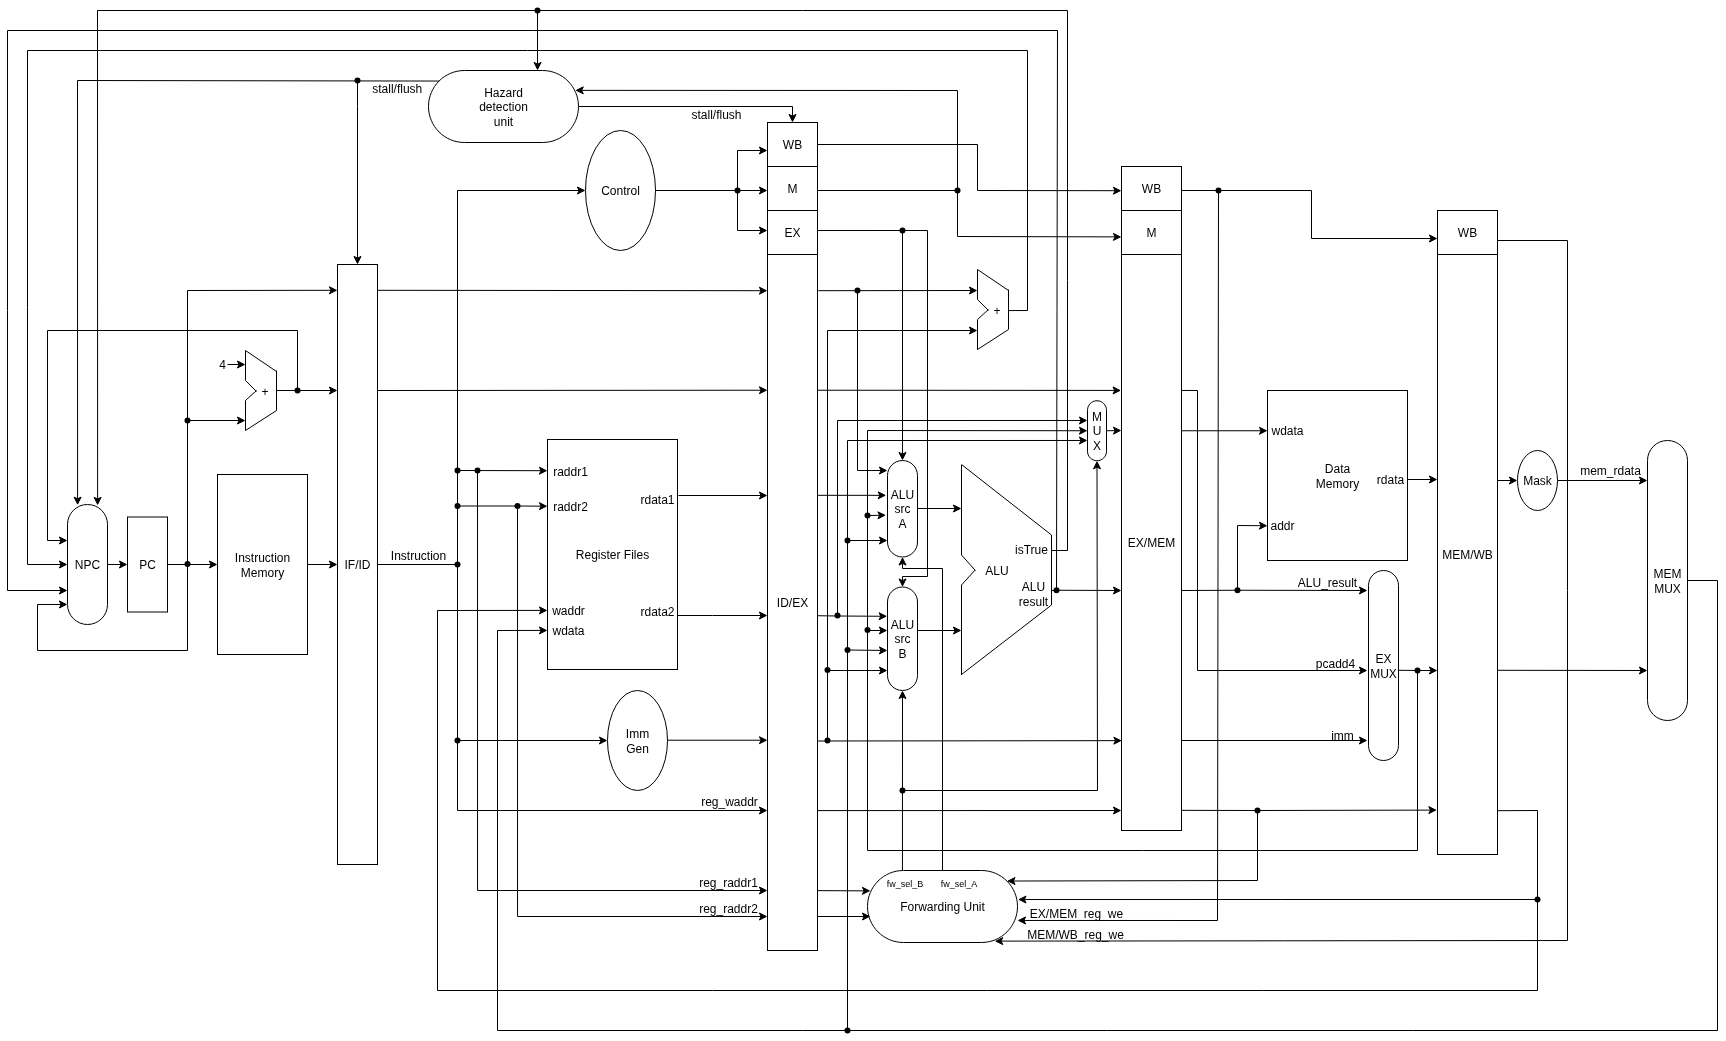
\includegraphics[width=1\textwidth]{CPU2.0 pipeline.drawio.png}
	\caption{CPU整体架构图}
\end{figure}

\newpage

\section{项目概述}

\subsection{项目背景}

RISC-V是一种开放的指令集架构，具有结构简洁、模块化程度高、扩展性强等特点，适合用于处理器设计教学、嵌入式系统开发和FPGA原型验证。本项目围绕``竞业达''企业命题初赛要求，基于RV32I基本整数指令集设计并实现一款32位CPU。通过该设计，可以完整训练从指令编码、数据通路、控制通路、流水线寄存器、冒险处理到FPGA接口适配的处理器设计流程。

本项目采用五级流水线结构，将指令执行过程划分为取指、译码、执行、访存和写回五个阶段。与单周期CPU相比，五级流水线能够在不同阶段并行处理多条指令，提高指令吞吐率；同时，流水线结构也引入了数据冒险和控制冒险问题，使得本设计进一步实现了前递单元和冒险检测单元，以保证程序执行结果的正确性。

\subsection{设计目标}

本项目的设计目标如下：

\begin{enumerate}
	\item 实现一款基于RV32I基本整数指令集的32位CPU；
	\item 采用五级流水线结构，实现IF、ID、EX、MEM、WB五个阶段；
	\item 支持初赛要求的37条RV32I基础指令；
	\item 完成PC更新、指令译码、立即数生成、寄存器读写、ALU运算、访存和写回等功能；
	\item 实现数据前递、load-use暂停和控制冒险冲刷机制；

\end{enumerate}

\subsection{设计平台说明}

\begin{table}[H]
	\centering
	\caption{设计平台说明}
	\begin{tabularx}{\textwidth}{p{4cm}X}
		\toprule
		项目     & 内容                                               \\
		\midrule
		硬件平台   & {竞业达数字孪生平台}                                      \\
		FPGA器件 & {Xilinx Kintex-7}                                \\
		开发工具   & {Vivado 2023.2}                                  \\
		硬件描述语言 & SystemVerilog                                    \\
		仿真工具   & {Vivado Simulation、Verilator}                    \\
		CPU时钟  & 企业模板默认提供50MHz外设时钟，可通过PLL调整；本设计使用CPU时钟频率为{120MHz} \\
		工程顶层   & 企业模板顶层 + 自研\code{myCPU}核心                        \\
		生成文件   & {src0.bit, src1.bit, src2.bit}                   \\
		\bottomrule
	\end{tabularx}
\end{table}

\section{RISC-V CPU架构设计}

\subsection{RV32I指令集的支持情况}

本CPU面向RV32I基本整数指令集进行设计。初赛测试要求中，RV32I共40条基础指令，排除\code{fence}、\code{ecall}、\code{ebreak}三条后，最低要求实现37条指令。本设计按照该目标对R型、I型、Load、Store、Branch、U型和J型指令进行支持。

\begin{longtable}{p{3cm}p{8cm}p{3cm}}
	\caption{RV32I指令支持情况}                                                           \\
	\toprule
	指令类型     & 指令                                                          & 当前设计状态 \\
	\midrule
	\endfirsthead
	\toprule
	指令类型     & 指令                                                          & 当前设计状态 \\
	\midrule
	\endhead
	R型运算指令   & \code{add, sub, sll, slt, sltu, xor, srl, sra, or, and}     & 已完成    \\
	I型运算指令   & \code{addi, slti, sltiu, xori, ori, andi, slli, srli, srai} & 已完成    \\
	Load指令   & \code{lb, lh, lw, lbu, lhu}                                 & 已完成    \\
	Store指令  & \code{sb, sh, sw}                                           & 已完成    \\
	Branch指令 & \code{beq, bne, blt, bge, bltu, bgeu}                       & 已完成    \\
	U型指令     & \code{lui, auipc}                                           & 已完成    \\
	J型指令     & \code{jal, jalr}                                            & 已完成    \\
	\bottomrule
\end{longtable}

\subsection{RV32I CPU的整体架构图}

本设计采用五级流水线结构。整体架构由取指阶段、译码阶段、执行阶段、访存阶段和写回阶段组成，各阶段之间通过流水线寄存器传递数据与控制信号。
\begin{figure}[H]
	\centering
	\resizebox{0.96\textwidth}{!}{
		\begin{tikzpicture}[
			font=\small,
			stage/.style={
					draw,
					rounded corners,
					minimum width=1.65cm,
					minimum height=0.9cm,
					align=center,
					thick
				},
			reg/.style={
					draw,
					minimum width=0.75cm,
					minimum height=0.75cm,
					align=center,
					font=\scriptsize
				},
			unit/.style={
					draw,
					rounded corners,
					minimum width=2.05cm,
					minimum height=0.65cm,
					align=center,
					font=\scriptsize
				},
			hazard/.style={
					draw,
					rounded corners,
					minimum width=3.2cm,
					minimum height=0.65cm,
					align=center,
					font=\scriptsize
				},
			dataarrow/.style={
			-{Stealth[length=2mm]},
			thick
			},
			ctrlarrow/.style={
			-{Stealth[length=2mm]},
			dashed,
			thick,
			rounded corners=3pt
			}
			]

			% ================= 主流水线阶段 =================
			\node[stage] (IF) at (0,0) {IF\\取指};
			\node[reg]   (IFID) at (1.75,0) {IF/ID};
			\node[stage] (ID) at (3.50,0) {ID\\译码};
			\node[reg]   (IDEX) at (5.25,0) {ID/EX};
			\node[stage] (EX) at (7.00,0) {EX\\执行};
			\node[reg]   (EXMEM) at (8.85,0) {EX/MEM};
			\node[stage] (MEM) at (10.75,0) {MEM\\访存};
			\node[reg]   (MEMWB) at (12.65,0) {MEM/WB};
			\node[stage] (WB) at (14.40,0) {WB\\写回};

			% ================= 主数据通路 =================
			\draw[dataarrow] (IF.east) -- (IFID.west);
			\draw[dataarrow] (IFID.east) -- (ID.west);
			\draw[dataarrow] (ID.east) -- (IDEX.west);
			\draw[dataarrow] (IDEX.east) -- (EX.west);
			\draw[dataarrow] (EX.east) -- (EXMEM.west);
			\draw[dataarrow] (EXMEM.east) -- (MEM.west);
			\draw[dataarrow] (MEM.east) -- (MEMWB.west);
			\draw[dataarrow] (MEMWB.east) -- (WB.west);

			% ================= 各阶段内部模块 =================
			\node[unit] (ifunit) at (0,-1.45) {PC / NPC\\IROM接口};
			\node[unit] (idunit) at (3.50,-1.45) {Control\\IMMGEN / RegFile};
			\node[unit] (exunit) at (7.00,-1.45) {ALU\\ALU\_src};
			\node[unit] (memunit) at (10.75,-1.45) {DRAM/外设接口\\Mask};
			\node[unit] (wbunit) at (14.40,-1.45) {写回选择\\RegFile写入};

			% 各阶段模块到对应流水线阶段，短虚线，不跨框
			\draw[ctrlarrow] (ifunit.north) -- (IF.south);
			\draw[ctrlarrow] (idunit.north) -- (ID.south);
			\draw[ctrlarrow] (exunit.north) -- (EX.south);
			\draw[ctrlarrow] (memunit.north) -- (MEM.south);
			\draw[ctrlarrow] (wbunit.north) -- (WB.south);

			% ================= 冒险处理单元 =================
			\node[hazard] (hazardunit) at (7.00,-2.85) {Forwarding Unit\\Hazard Detection Unit};

			% 冒险处理到EX阶段，短虚线
			\draw[ctrlarrow] (hazardunit.north) -- (exunit.south);

			% 冒险处理到IF/ID，路线从底部绕行，不压框
			\draw[ctrlarrow]
			(hazardunit.west)
			-- (1.75,-2.85)
			-- (IFID.south);

			% 冒险处理到ID/EX，路线走模块间隙，不压框
			\draw[ctrlarrow]
			(hazardunit.west)
			-- (5.25,-3.25)
			-- (IDEX.south);

			% 写回反馈到寄存器堆，从右侧绕到底部，不穿过中间框图
			\draw[ctrlarrow]
			(WB.east)
			-- ++(0.45,0)
			|- (3.50,-4.05)
			-- (idunit.south);

		\end{tikzpicture}
	}
	\caption{五级流水线 CPU 整体架构示意图}
	\label{fig:cpu_arch}
\end{figure}
本设计采用哈佛式存储结构，指令访问接口与数据/外设访问接口相互独立。取指阶段通过 \texttt{irom\_addr} 和 \texttt{irom\_data} 访问 IROM；访存阶段通过 \texttt{perip\_addr}、\texttt{perip\_wen}、\texttt{perip\_mask}、\texttt{perip\_wdata} 和 \texttt{perip\_rdata} 访问 DRAM 或外设。因此，IF 阶段取指和 MEM 阶段访存可以在接口层面分离，符合五级流水线 CPU 的设计需求。

这种结构使取指通路和数据访存通路在接口层面相互独立，便于五级流水线中 IF 阶段和 MEM 阶段分别完成指令读取与数据访问，降低指令存储器访问和数据存储器访问之间的结构冲突风险，也更符合企业提供工程模板中 IROM、DRAM 与外设分离的系统结构。图~\ref{fig:cpu_arch} 中实线表示主流水线数据通路，虚线表示控制、前递、暂停、冲刷和写回相关通路。

\begin{figure}[H]
	\centering
	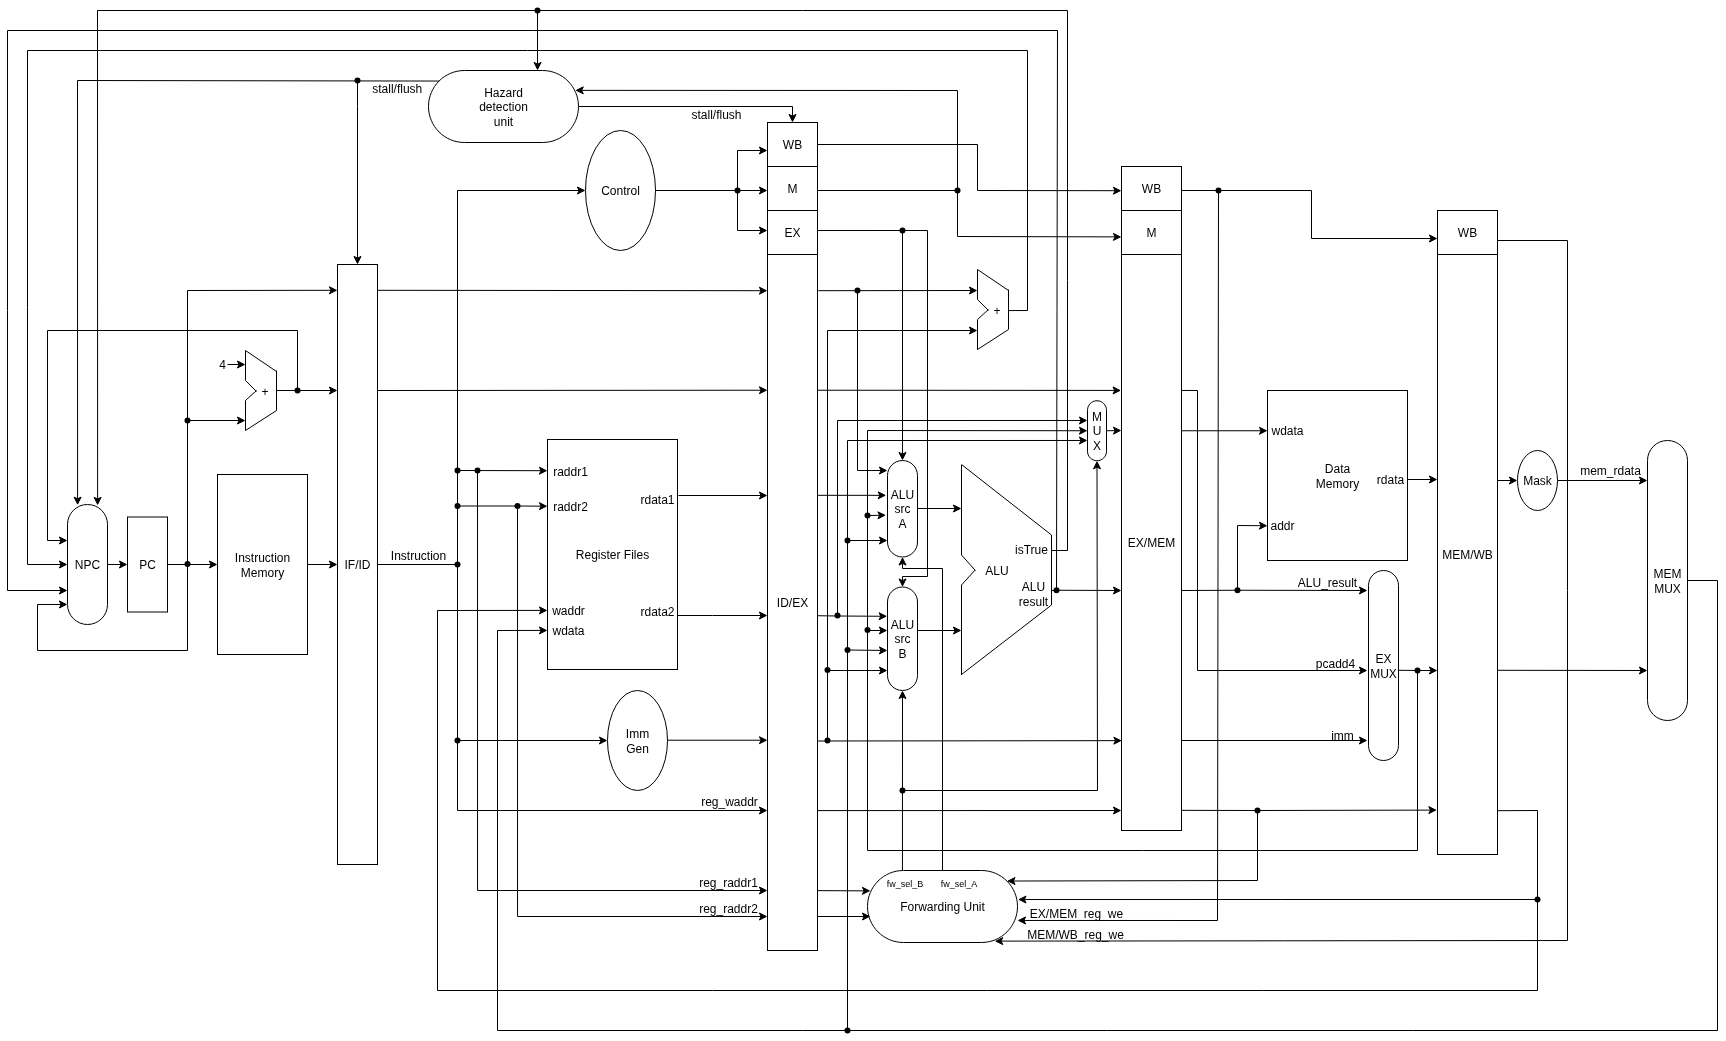
\includegraphics[width=1\textwidth]{CPU2.0 pipeline.drawio.png}
	\caption{CPU RTL结构图}
\end{figure}

\subsection{CPU顶层接口设计}

本CPU顶层模块为\code{myCPU}，源文件位于企业工程的\code{digital\_twin.srcs/sources\_1/imports/news/}目录下。该模块通过系统时钟复位、IROM指令存储器接口以及DRAM/外设统一接口接入企业提供的工程模板。

\begin{table}[H]
\centering
\caption{\code{myCPU}顶层接口说明}
\begin{tabularx}{\textwidth}{p{3cm}p{2cm}p{2cm}X}
\toprule
信号名称 & 方向 & 位宽 & 功能说明 \\
\midrule
\code{cpu\_clk} & input & 1 & CPU工作时钟 \\
\code{cpu\_rst} & input & 1 & CPU复位信号 \\
\code{irom\_addr} & output & 32 & 指令存储器访问地址，由当前PC给出 \\
\code{irom\_data} & input & 32 & 指令存储器返回的32位指令 \\
\code{perip\_addr} & output & 32 & DRAM或外设访问地址，由MEM阶段传递的ALU结果给出 \\
\code{perip\_wen} & output & 1 & 写使能信号，Store指令有效 \\
\code{perip\_mask} & output & 2 & 访存宽度控制，00表示1字节，01表示2字节，10表示4字节 \\
\code{perip\_wdata} & output & 32 & 写入DRAM或外设的数据 \\
\code{perip\_rdata} & input & 32 & DRAM或外设返回的数据 \\
\bottomrule
\end{tabularx}
\end{table}


\subsection{地址空间与外设访问方式}

根据企业提供的工程模板，CPU 通过独立的 IROM 接口访问指令存储器，通过统一的 \code{perip} 接口访问 DRAM 和外设地址空间。CPU 核心只负责输出访问地址、写使能、访问宽度和写入数据，具体地址译码由模板中的外部平台完成。因此，CPU 内部数据通路可以保持相对独立，不需要将数码管、LED 或按键等外设的译码逻辑写入 CPU 核心。

\begin{table}[H]
	\centering
	\caption{企业平台地址空间映射}
	\footnotesize
	\renewcommand{\arraystretch}{1.2}
	\begin{tabularx}{\textwidth}{p{3cm}p{4.2cm}X}
		\toprule
		区域      & 地址范围                              & 功能说明                                  \\
		\midrule
		IROM    & \code{0x8000\_0000--0x800F\_FFFF} & 指令存储器地址空间，其中前 16KB 用于 IROM 初始化程序，只读。  \\
		DRAM    & \code{0x8010\_0000--0x801F\_FFFF} & 数据存储器地址空间，其中前 256KB 用于 DRAM 初始化与读写访问。 \\
		SW      & \code{0x8020\_0000--0x8020\_0007} & 开关输入区域，只读，用于读取开关状态。                   \\
		KEY     & \code{0x8020\_0010--0x8020\_0013} & 按键输入区域，只读，用于读取按键状态。                   \\
		SEG     & \code{0x8020\_0020--0x8020\_0023} & 七段数码管显示区域，读写，用于显示测试结果。                \\
		LED     & \code{0x8020\_0040--0x8020\_0043} & LED 显示区域，只写，用于显示测试状态或结果。              \\
		COUNTER & \code{0x8020\_0050--0x8020\_0053} & 计数器区域，读写，用于记录测试程序运行时间。                \\
		\bottomrule
	\end{tabularx}
\end{table}

在访存类指令执行时，ALU 计算出的地址通过 \code{perip\_addr} 输出。对于 Store 指令，\code{perip\_wen} 置位，\code{perip\_mask} 指示写入宽度，\code{perip\_wdata} 输出待写入数据；对于 Load 指令，外部平台将读出数据通过 \code{perip\_rdata} 返回 CPU，并在后续写回阶段由 \code{Mask} 模块完成符号扩展或零扩展。

\subsection{数据通路各模块的设计}

\subsubsection{PC模块}

\code{PC}模块用于保存当前取指地址。复位时，正常上板模式下PC初始化为\code{0x8000\_0000}，以匹配企业模板中IROM起始地址；开启\code{ENABLE\_DEBUG\_TRACE}调试宏时，复位值为\code{0x0000\_0000}，便于trace仿真跟踪。正常运行时，PC在时钟上升沿更新为\code{NPC}模块生成的下一条指令地址。

\begin{table}[H]
\centering
\caption{\code{PC}模块输入输出信号说明}
\footnotesize
\renewcommand{\arraystretch}{1.15}
\begin{tabularx}{\textwidth}{p{3.2cm}p{1.5cm}p{2.1cm}X}
\toprule
参数名 & 方向 & 位宽 & 说明 \\
\midrule
\code{clk} & 输入 & 1 & 系统时钟信号，上升沿更新PC寄存器。 \\
\code{rst} & 输入 & 1 & 复位信号，复位时PC回到参数\code{RESET\_VAL}。 \\
\code{npc} & 输入 & 32 & NPC模块计算得到的下一条指令地址。 \\
\code{pc} & 输出 & 32 & 当前取指地址，连接到IROM地址端口。 \\
\bottomrule
\end{tabularx}
\end{table}

\subsubsection*{设计细节}

PC 模块的输入信号包括系统时钟、复位信号和下一条指令地址 \code{npc}，输出信号为当前取指地址 \code{pc}。模块内部使用寄存器保存当前 PC 值，在时钟上升沿将其更新为 NPC 模块计算得到的下一地址。

该模块只负责保存和更新 PC，不直接判断分支或跳转条件。这样可以将“当前 PC 状态保存”和“下一 PC 选择”分离：PC 模块负责时序寄存，NPC 模块负责组合选择。该划分使 PC 更新路径更加清晰，也便于在仿真中分别观察 PC 当前值和 NPC 目标值。

\subsubsection{NPC模块}

\code{NPC}模块根据\code{npc\_op}选择下一条PC地址。\code{npc\_op=00}表示顺序执行或stall保持，\code{npc\_op=01}表示条件分支，\code{npc\_op=10}表示\code{jalr}，\code{npc\_op=11}表示\code{jal}。对于\code{jalr}，模块将ALU计算结果最低位置零，以符合RISC-V对\code{jalr}目标地址的要求。

\begin{table}[H]
\centering
\caption{\code{NPC}模块输入输出信号说明}
\footnotesize
\renewcommand{\arraystretch}{1.15}
\begin{tabularx}{\textwidth}{p{3.2cm}p{1.5cm}p{2.1cm}X}
\toprule
参数名 & 方向 & 位宽 & 说明 \\
\midrule
\code{isTrue} & 输入 & 1 & ALU输出的分支条件判断结果。 \\
\code{stall} & 输入 & 1 & 流水线暂停信号，有效时保持当前PC。 \\
\code{npc\_op} & 输入 & 2 & 下一PC选择信号：顺序/分支/\code{jalr}/\code{jal}。 \\
\code{pc} & 输入 & 32 & 当前PC值。 \\
\code{pc\_add\_4} & 输入 & 32 & 顺序执行时的\code{PC+4}。 \\
\code{pc\_add\_imm} & 输入 & 32 & 分支或\code{jal}目标地址\code{PC+imm}。 \\
\code{alu\_result} & 输入 & 32& \code{jalr}指令由ALU计算出的\code{rs1+imm}。 \\
\code{npc} & 输出 & 32 & 送回PC模块的下一条指令地址。 \\
\bottomrule
\end{tabularx}
\end{table}

\subsubsection*{设计细节}

NPC 模块的输入包括当前 PC、\code{PC+4}、\code{PC+imm}、ALU 计算结果、分支判断结果 \code{isTrue}、流水线暂停信号 \code{stall} 和下一 PC 选择信号 \code{npc\_op}。输出为下一周期将要写入 PC 模块的 \code{npc}。

当 \code{stall} 有效时，NPC 输出当前 PC，使取指阶段保持不变；当 \code{npc\_op=00} 时，CPU 默认顺序执行，下一地址为 \code{PC+4}；当 \code{npc\_op=01} 时，NPC 根据分支条件选择 \code{PC+imm} 或 \code{PC+4}；当 \code{npc\_op=10} 时，NPC 选择 \code{jalr} 的 ALU 计算结果并对齐；当 \code{npc\_op=11} 时，NPC 选择 \code{jal} 的目标地址。通过该模块，顺序执行、条件分支和无条件跳转被统一到同一条 PC 更新路径中。

\subsubsection{IF/ID流水线寄存器}

\code{IF\_ID}模块连接IF与ID阶段，保存取指阶段得到的PC、PC+4和指令。当发生\code{stall}时保持原值，当发生\code{flush}时清空寄存器内容，用于处理load-use冒险和控制冒险。

\begin{table}[H]
\centering
\caption{\code{IF\_ID}流水线寄存器输入输出信号说明}
\footnotesize
\renewcommand{\arraystretch}{1.15}
\begin{tabularx}{\textwidth}{p{3.2cm}p{1.5cm}p{2.1cm}X}
\toprule
参数名 & 方向 & 位宽 & 说明 \\
\midrule
\code{clk} & 输入 & 1 & 系统时钟信号。 \\
\code{rst} & 输入 & 1 & 复位信号。 \\
\code{stall} & 输入 & 1 & 暂停信号，有效时保持当前寄存器值。 \\
\code{flush} & 输入 & 1 & 冲刷信号，有效时清空输出。 \\
\code{if\_pc} & 输入 & 32 & IF阶段当前PC。 \\
\code{if\_pc4} & 输入 & 32 & IF阶段计算得到的\code{PC+4}。 \\
\code{if\_instr} & 输入 & 32 & IF阶段从IROM读出的指令。 \\
\code{id\_pc} & 输出 & 32 & 传递到ID阶段的PC。 \\
\code{id\_pc4} & 输出 & 32 & 传递到ID阶段的\code{PC+4}。 \\
\code{id\_instr} & 输出 & 32 & 传递到ID阶段的指令。 \\
\bottomrule
\end{tabularx}
\end{table}

\subsubsection*{设计细节}

IF/ID 流水线寄存器的输入来自 IF 阶段，包括当前指令地址、\code{PC+4} 和从 IROM 读出的指令；输出送往 ID 阶段，用于译码、寄存器读取和立即数生成。

当 \code{stall} 有效时，该模块保持原值，避免当前处于 ID 阶段的指令被新取出的指令覆盖；当 \code{flush} 有效时，该模块清空输出，相当于向流水线中插入空操作。该控制方式使取指阶段能够配合 load-use 暂停和分支/跳转冲刷机制。

\subsubsection{Control控制模块}

\code{Control}模块根据指令\code{opcode}和\code{funct3/funct7}字段产生控制信号。当前控制器可识别R型、I型、Load、Store、Branch、U型和J型指令，输出包括\code{NpcOp}、\code{RegWrite}、\code{MemToReg\_sel}、\code{MemWrite}、\code{ALUSrcA}、\code{ALUSrcB}、\code{ALUControl}和\code{mask}等控制信号。

\begin{table}[H]
\centering
\caption{\code{Control}模块输入输出信号说明}
\footnotesize
\renewcommand{\arraystretch}{1.15}
\begin{tabularx}{\textwidth}{p{3.2cm}p{1.5cm}p{2.1cm}X}
\toprule
参数名 & 方向 & 位宽 & 说明 \\
\midrule
\code{instr} & 输入 & 32 & 当前32位指令。 \\
\code{NpcOp} & 输出 & 2 & 下一PC选择控制信号。 \\
\code{RegWrite} & 输出 & 1 & 寄存器堆写使能信号。 \\
\code{MemToReg\_sel} & 输出 & 2 & 写回来源选择信号。 \\
\code{MemWrite} & 输出 & 1 & DRAM/外设写使能信号。 \\
\code{ALUSrcA} & 输出 & 1 & ALU第一个操作数来源选择。 \\
\code{ALUSrcB} & 输出 & 1 & ALU第二个操作数来源选择。 \\
\code{ALUControl} & 输出 & 14 & ALU运算控制信号。 \\
\code{mask} & 输出 & 3 & 访存宽度及load扩展控制，来自\code{funct3}。 \\
\bottomrule
\end{tabularx}
\end{table}

\subsubsection*{设计细节}

Control 模块输入为完整的 32 位指令。模块首先提取低 7 位 \code{opcode} 判断指令大类，再结合 \code{funct3} 和 \code{funct7[5]} 判断具体运算类型。对于 R 型和 I 型运算指令，控制器根据 funct 字段产生对应的 ALU 运算控制；对于 Load、Store 和 \code{jalr} 指令，ALU 执行加法用于地址计算；对于 Branch 指令，ALU 执行条件比较；对于 \code{lui}，写回来源选择立即数；对于 \code{jal} 和 \code{jalr}，写回来源选择 \code{PC+4}。

本设计中的 \code{ALUControl} 为 14 位控制信号，不同控制位对应加法、减法、逻辑运算、移位运算和条件比较等操作。与再次二级译码相比，这种控制方式使 ALU 内部能够直接根据控制位选择结果，逻辑关系直观，便于后续调试。

\subsubsection{IMMGEN立即数生成模块}

\code{IMMGEN}模块根据指令格式生成立即数。支持I型、S型、B型、U型和J型立即数，并按照RISC-V编码规则进行符号扩展和位拼接。其中B型和J型立即数最低位补0，以适配分支和跳转指令的目标地址计算。

\begin{table}[H]
\centering
\caption{\code{IMMGEN}模块输入输出信号说明}
\footnotesize
\renewcommand{\arraystretch}{1.15}
\begin{tabularx}{\textwidth}{p{3.2cm}p{1.5cm}p{2.1cm}X}
\toprule
参数名 & 方向 & 位宽 & 说明 \\
\midrule
\code{instr} & 输入 & 32 & 当前32位指令。 \\
\code{imm} & 输出 & 32 & 按指令类型生成并符号扩展后的立即数。 \\
\bottomrule
\end{tabularx}
\end{table}

\subsubsection*{设计细节}

IMMGEN 模块的输入为 32 位指令，输出为扩展后的 32 位立即数。I 型立即数来自 \code{instr[31:20]}；S 型立即数由 \code{instr[31:25]} 和 \code{instr[11:7]} 拼接；B 型立即数按照分支指令的编码位置重排并补最低位 0；U 型立即数由高 20 位左移形成；J 型立即数按照 \code{jal} 的编码格式拼接，并同样补最低位 0。

由于 RV32I 各类指令的立即数字段分布不同，将立即数生成集中到 IMMGEN 模块可以避免后续模块重复解析指令字段，也使数据通路中与立即数相关的路径更加统一。

\subsubsection{RegFile寄存器堆模块}

\code{RegFile}模块包含32个32位通用寄存器，支持两个读端口和一个写端口。写回阶段当\code{wen}有效且\code{waddr}不为0时写入寄存器。模块中还实现了同周期读写同一寄存器时的内部旁路逻辑，若读地址与写地址相同，则读端口优先返回当前写入数据。

\begin{table}[H]
\centering
\caption{\code{RegFile}模块输入输出信号说明}
\footnotesize
\renewcommand{\arraystretch}{1.15}
\begin{tabularx}{\textwidth}{p{3.2cm}p{1.5cm}p{2.1cm}X}
\toprule
参数名 & 方向 & 位宽 & 说明 \\
\midrule
\code{clk} & 输入 & 1 & 系统时钟信号。 \\
\code{rst} & 输入 & 1 & 复位信号。 \\
\code{wen} & 输入 & 1 & 写使能信号。 \\
\code{waddr} & 输入 & 5 & 写寄存器地址。 \\
\code{wdata} & 输入 & 32 & 写回数据。 \\
\code{rR1} & 输入 & 5 & 第一个读寄存器地址，对应\code{rs1}。 \\
\code{rR2} & 输入 & 5 & 第二个读寄存器地址，对应\code{rs2}。 \\
\code{rR1\_data} & 输出 & 32 & 第一个读端口输出数据。 \\
\code{rR2\_data} & 输出 & 32 & 第二个读端口输出数据。 \\
\bottomrule
\end{tabularx}
\end{table}

\subsubsection*{设计细节}

RegFile 模块输入包括读寄存器地址 \code{rs1}、\code{rs2}，写寄存器地址 \code{rd}，写回数据 \code{wdata} 和写使能 \code{wen}，输出为两个源寄存器读出值。寄存器 \code{x0} 在 RISC-V 中恒为 0，因此即使写地址为 0，也不会真正改变 \code{x0} 的值。

在五级流水线中，WB 阶段写回和 ID 阶段读寄存器可能发生在同一周期。为了避免 ID 阶段读取到旧值，本设计在寄存器堆中加入同周期读写旁路：当读地址与写地址相同且写使能有效时，读端口优先返回当前写回数据。该处理可以减少写回阶段与译码阶段之间的读写相关。

\subsubsection{ID/EX流水线寄存器}

\code{ID\_EX}模块连接ID与EX阶段，传递PC、PC+4、源寄存器值、立即数、源/目的寄存器编号以及执行、访存和写回相关控制信号。当发生\code{id\_stall}或\code{id\_flush}时，模块将写使能、访存写使能、NPC控制等关键控制信号清零，从而在EX阶段插入无效操作。

{\footnotesize
\renewcommand{\arraystretch}{1.12}
\begin{longtable}{p{3.2cm}p{1.5cm}p{2.1cm}p{7.0cm}}
\caption{\code{ID\_EX}流水线寄存器输入输出信号说明}\\
\toprule
参数名 & 方向 & 位宽 & 说明 \\
\midrule
\endfirsthead
\toprule
参数名 & 方向 & 位宽 & 说明 \\
\midrule
\endhead
\code{clk} & 输入 & 1 & 系统时钟信号。 \\
\code{rst} & 输入 & 1 & 复位信号。 \\
\code{id\_stall} & 输入 & 1 & ID/EX暂停控制信号。 \\
\code{id\_flush} & 输入 & 1 & ID/EX冲刷控制信号。 \\
\code{id\_pc} & 输入 & 32 & ID阶段PC。 \\
\code{id\_pc4} & 输入 & 32 & ID阶段\code{PC+4}。 \\
\code{id\_rs1v} & 输入 & 32 & 寄存器堆读出的\code{rs1}数据。 \\
\code{id\_rs2v} & 输入 & 32 & 寄存器堆读出的\code{rs2}数据。 \\
\code{id\_imm} & 输入 & 32 & 立即数生成模块输出。 \\
\code{id\_rs1} & 输入 & 5 & 源寄存器\code{rs1}编号。 \\
\code{id\_rs2} & 输入 & 5 & 源寄存器\code{rs2}编号。 \\
\code{id\_rd} & 输入 & 5 & 目的寄存器\code{rd}编号。 \\
\code{id\_alu\_op} & 输入 & 14 & ID阶段产生的ALU控制信号。 \\
\code{id\_alusrcA} & 输入 & 1 & ALU输入A来源控制。 \\
\code{id\_alusrcB} & 输入 & 1 & ALU输入B来源控制。 \\
\code{id\_npcop} & 输入 & 2 & 下一PC控制信号。 \\
\code{id\_mem\_write} & 输入 & 1 & 访存写使能控制信号。 \\
\code{id\_mask} & 输入 & 3 & 访存宽度及扩展控制信号。 \\
\code{id\_regwrmux} & 输入 & 2 & 写回来源选择信号。 \\
\code{id\_reg\_write} & 输入 & 1 & 寄存器写使能信号。 \\
\code{ex\_pc} & 输出 & 32 & 传递到EX阶段的PC。 \\
\code{ex\_pc4} & 输出 & 32 & 传递到EX阶段的\code{PC+4}。 \\
\code{ex\_rs1v} & 输出 & 32 & EX阶段使用的\code{rs1}数据。 \\
\code{ex\_rs2v} & 输出 & 32 & EX阶段使用的\code{rs2}数据。 \\
\code{ex\_imm} & 输出 & 32 & EX阶段使用的立即数。 \\
\code{ex\_rs1} & 输出 & 5 & EX阶段\code{rs1}编号。 \\
\code{ex\_rs2} & 输出 & 5 & EX阶段\code{rs2}编号。 \\
\code{ex\_rd} & 输出 & 5 & EX阶段目的寄存器编号。 \\
\code{ex\_alu\_op} & 输出 & 14 & EX阶段ALU控制信号。 \\
\code{ex\_alusrcA} & 输出 & 1 & EX阶段ALU输入A选择。 \\
\code{ex\_alusrcB} & 输出 & 1 & EX阶段ALU输入B选择。 \\
\code{ex\_npcop} & 输出 & 2 & EX阶段下一PC控制。 \\
\code{ex\_mem\_write} & 输出 & 1 & EX阶段访存写使能。 \\
\code{ex\_mask} & 输出 & 3 & EX阶段访存宽度及扩展控制。 \\
\code{ex\_regwrmux} & 输出 & 2 & EX阶段写回来源选择。 \\
\code{ex\_reg\_write} & 输出 & 1 & EX阶段寄存器写使能。 \\
\bottomrule
\end{longtable}
}

\subsubsection*{设计细节}

ID/EX 流水线寄存器保存译码阶段产生的主要数据，包括 \code{PC}、\code{PC+4}、寄存器堆读出的 \code{rs1} 和 \code{rs2} 数据、立即数、源寄存器编号、目的寄存器编号，以及控制器产生的执行、访存和写回控制信号。

该模块不仅传递数据，也承担插入气泡的作用。当检测到 load-use 冒险或控制冒险时，ID/EX 将可能产生副作用的控制信号清零，例如寄存器写使能、访存写使能和 PC 跳转控制信号，从而保证错误路径或等待数据的指令不会继续修改系统状态。

\subsubsection{ALU\_src操作数选择模块}

\code{ALU\_src}模块用于选择ALU输入操作数。若\code{alu\_src}为1，则选择立即数或PC；若为0，则根据前递选择信号在寄存器原始值、MEM阶段结果和WB阶段写回数据中选择正确操作数。

\begin{table}[H]
\centering
\caption{\code{ALU\_src}模块输入输出信号说明}
\footnotesize
\renewcommand{\arraystretch}{1.15}
\begin{tabularx}{\textwidth}{p{3.2cm}p{1.5cm}p{2.1cm}X}
\toprule
参数名 & 方向 & 位宽 & 说明 \\
\midrule
\code{alu\_src} & 输入 & 1 & 操作数来源选择，决定是否直接选择\code{alusrc1}。 \\
\code{forward\_src} & 输入 & 2 & 前递选择信号。 \\
\code{alusrc0} & 输入 & 32 & 寄存器原始操作数。 \\
\code{alusrc1} & 输入 & 32 & 立即数或PC候选操作数。 \\
\code{fwdsrc0} & 输入 & 32 & MEM阶段前递数据。 \\
\code{fwdsrc1} & 输入 & 32 & WB阶段前递数据。 \\
\code{result} & 输出 & 32 & 最终送入ALU的操作数。 \\
\bottomrule
\end{tabularx}
\end{table}

\subsubsection*{设计细节}

ALU\_src 模块的输入包括原始寄存器数据、立即数或 PC 候选数据、MEM 阶段前递数据、WB 阶段写回数据，以及来自 forwarding unit 的前递选择信号。该模块负责在 EX 阶段为 ALU 选择正确的两个操作数。

对于 R 型指令，两个操作数通常来自寄存器堆；对于 I 型运算、Load、Store 和 \code{jalr} 指令，第二个操作数来自立即数；对于 \code{auipc}，第一个操作数来自 PC。当前递单元检测到 RAW 数据相关时，ALU\_src 会优先选择来自 MEM 或 WB 阶段的最新结果，而不是寄存器堆中的旧值。

\subsubsection{ALU模块}

\code{ALU}模块使用14位\code{ALUControl}信号控制具体运算。支持加法、减法、按位与、按位或、按位异或、逻辑左移、逻辑右移、算术右移、有符号比较、无符号比较以及分支条件判断。分支判断结果通过\code{isTrue}输出给冒险检测单元和NPC模块。

\begin{table}[H]
\centering
\caption{\code{ALU}模块输入输出信号说明}
\footnotesize
\renewcommand{\arraystretch}{1.15}
\begin{tabularx}{\textwidth}{p{3.2cm}p{1.5cm}p{2.1cm}X}
\toprule
参数名 & 方向 & 位宽 & 说明 \\
\midrule
\code{A} & 输入 & 32 & ALU第一个操作数。 \\
\code{B} & 输入 & 32 & ALU第二个操作数。 \\
\code{ALUControl} & 输入 & 14 & ALU运算控制信号。 \\
\code{Result} & 输出 & 32 & ALU运算或比较结果。 \\
\code{isTrue} & 输出 & 1 & 分支判断结果，取\code{Result[0]}。 \\
\bottomrule
\end{tabularx}
\end{table}

\subsubsection*{设计细节}

ALU 模块输入为两个 32 位操作数和 14 位 \code{ALUControl} 控制信号，输出为 32 位运算结果 \code{Result} 和分支判断信号 \code{isTrue}。移位类指令使用第二操作数的低 5 位作为移位位数，符合 RV32I 对移位操作的定义。

对于普通算术逻辑指令，ALU 输出结果将通过后续流水线寄存器进入写回路径；对于 Load/Store 指令，ALU 的加法结果作为访存地址；对于 Branch 指令，ALU 输出比较结果，并通过 \code{isTrue} 指示分支是否成立。这样，普通运算、地址计算和分支判断共用同一个执行模块，减少了执行阶段硬件结构的重复。

\subsubsection{EX/MEM流水线寄存器}

\code{EX\_MEM}模块连接EX与MEM阶段，保存ALU结果、store写数据、立即数、PC+4、目的寄存器编号和访存/写回控制信号。进入MEM阶段后，ALU结果作为\code{perip\_addr}输出，store写数据作为\code{perip\_wdata}输出。

{\footnotesize
\renewcommand{\arraystretch}{1.12}
\begin{longtable}{p{3.2cm}p{1.5cm}p{2.1cm}p{7.0cm}}
\caption{\code{EX\_MEM}流水线寄存器输入输出信号说明}\\
\toprule
参数名 & 方向 & 位宽 & 说明 \\
\midrule
\endfirsthead
\toprule
参数名 & 方向 & 位宽 & 说明 \\
\midrule
\endhead
\code{clk} & 输入 & 1 & 系统时钟信号。 \\
\code{rst} & 输入 & 1 & 复位信号。 \\
\code{ex\_alu\_result} & 输入 & 32 & EX阶段ALU结果。 \\
\code{ex\_rs2\_val} & 输入 & 32 & EX阶段传入的\code{rs2}值，用于Store写数据。 \\
\code{ex\_imm} & 输入 & 32 & EX阶段立即数。 \\
\code{ex\_pc4} & 输入 & 32 & EX阶段\code{PC+4}。 \\
\code{ex\_rd\_addr} & 输入 & 5 & EX阶段目的寄存器编号。 \\
\code{ex\_mask} & 输入 & 3 & EX阶段访存宽度及扩展控制。 \\
\code{ex\_regwrmux} & 输入 & 2 & EX阶段写回来源选择。 \\
\code{ex\_reg\_write} & 输入 & 1 & EX阶段寄存器写使能。 \\
\code{ex\_mem\_write} & 输入 & 1 & EX阶段访存写使能。 \\
\code{mem\_alu\_result} & 输出 & 32 & MEM阶段ALU结果。 \\
\code{mem\_rs2\_val} & 输出 & 32 & MEM阶段Store写数据。 \\
\code{mem\_imm} & 输出 & 32 & MEM阶段立即数。 \\
\code{mem\_pc4} & 输出 & 32 & MEM阶段\code{PC+4}。 \\
\code{mem\_rd\_addr} & 输出 & 5 & MEM阶段目的寄存器编号。 \\
\code{mem\_mask} & 输出 & 3 & MEM阶段访存宽度及扩展控制。 \\
\code{mem\_regwrmux} & 输出 & 2 & MEM阶段写回来源选择。 \\
\code{mem\_reg\_write} & 输出 & 1 & MEM阶段寄存器写使能。 \\
\code{mem\_mem\_write} & 输出 & 1 & MEM阶段访存写使能。 \\
\bottomrule
\end{longtable}
}

\subsubsection*{设计细节}

EX/MEM 流水线寄存器保存执行阶段的计算结果和后续访存/写回需要的信息。对于 R 型和 I 型运算指令，ALU 结果继续传递到写回路径；对于 Load/Store 指令，ALU 结果作为 DRAM 或外设访问地址；对于 Store 指令，\code{rs2} 的值继续传递为 \code{perip\_wdata}。

该模块还传递目的寄存器编号和寄存器写使能等信号，供 MEM 阶段和 forwarding unit 判断是否需要向 EX 阶段前递数据。

\subsubsection{ex\_mux与mem\_mux模块}

\code{ex\_mux}用于在MEM阶段预先选择写回候选结果，包括PC+4、ALU结果和立即数。\code{mem\_mux}用于在WB阶段最终选择写回数据，当\code{regwrmux=10}时选择经过\code{Mask}处理的load数据，否则选择\code{ex\_mux}输出。

\begin{table}[H]
\centering
\caption{\code{ex\_mux}与\code{mem\_mux}模块输入输出信号说明}
\footnotesize
\renewcommand{\arraystretch}{1.15}
\begin{tabularx}{\textwidth}{p{3.2cm}p{1.5cm}p{2.1cm}X}
\toprule
参数名 & 方向 & 位宽 & 说明 \\
\midrule
\code{pcadd4} & 输入 & 32 & \code{ex\_mux}输入，跳转链接指令写回候选值。 \\
\code{imm} & 输入 & 32 & \code{ex\_mux}输入，\code{lui}写回候选值。 \\
\code{alu} & 输入 & 32 & \code{ex\_mux}输入，ALU结果写回候选值。 \\
\code{ex\_mux.result} & 输出 & 32 & \code{ex\_mux}输出的非Load类写回候选值。 \\
\code{ex\_mux} & 输入 & 32 & \code{mem\_mux}输入，来自\code{ex\_mux}的候选值。 \\
\code{mdata} & 输入 & 32 & \code{mem\_mux}输入，经过Mask处理的Load数据。 \\
\code{alu\_mux} & 输入 & 2 & 写回来源选择信号。 \\
\code{mem\_mux.result} & 输出 & 32 & WB阶段最终写回数据。 \\
\bottomrule
\end{tabularx}
\end{table}

\subsubsection*{设计细节}

ex\_mux 根据写回选择信号在 MEM 阶段预先选择非 load 类指令的写回候选值。\code{jal} 和 \code{jalr} 选择 \code{PC+4}，R 型、I 型和 \code{auipc} 选择 ALU 结果，\code{lui} 选择立即数。

mem\_mux 位于 WB 阶段，用于区分 load 指令和其他写回指令。当写回选择信号表示访存数据时，mem\_mux 选择经过 Mask 处理的 load 数据；否则选择 ex\_mux 产生的候选值。通过这种两级选择方式，执行阶段结果和访存读出结果的写回路径更加清晰。

\subsubsection{Mask模块}

\code{Mask}模块用于处理load指令读出的数据。对于\code{lb}和\code{lh}执行符号扩展，对于\code{lbu}和\code{lhu}执行零扩展，对于\code{lw}直接保留32位数据。

\begin{table}[H]
\centering
\caption{\code{Mask}模块输入输出信号说明}
\footnotesize
\renewcommand{\arraystretch}{1.15}
\begin{tabularx}{\textwidth}{p{3.2cm}p{1.5cm}p{2.1cm}X}
\toprule
参数名 & 方向 & 位宽 & 说明 \\
\midrule
\code{mask} & 输入 & 3 & Load指令类型及扩展方式控制。 \\
\code{dout} & 输入 & 32 & DRAM/外设读出的原始32位数据。 \\
\code{mdata} & 输出 & 32 & 符号扩展或零扩展后的32位写回数据。 \\
\bottomrule
\end{tabularx}
\end{table}

\subsubsection*{设计细节}

Mask 模块输入包括访存控制信号 \code{mask} 和从 DRAM/外设读出的原始数据，输出为处理后的 32 位写回数据。对于 \code{lb}，模块取低 8 位并按照符号位扩展到 32 位；对于 \code{lh}，取低 16 位并符号扩展；对于 \code{lbu} 和 \code{lhu}，则分别进行 8 位和 16 位零扩展；对于 \code{lw}，直接保留 32 位数据。

该模块保证了不同 load 指令虽然访问宽度不同，但最终都能形成符合 RV32I 语义的 32 位写回数据。

\subsubsection{MEM/WB流水线寄存器}

\code{MEM\_WB}模块连接MEM与WB阶段，保存访存读数据、MEM阶段写回候选结果、目的寄存器编号以及写回控制信号。WB阶段根据选择结果将数据写回寄存器堆。

{\footnotesize
\renewcommand{\arraystretch}{1.12}
\begin{longtable}{p{3.2cm}p{1.5cm}p{2.1cm}p{7.0cm}}
\caption{\code{MEM\_WB}流水线寄存器输入输出信号说明}\\
\toprule
参数名 & 方向 & 位宽 & 说明 \\
\midrule
\endfirsthead
\toprule
参数名 & 方向 & 位宽 & 说明 \\
\midrule
\endhead
\code{mem\_pc4} & 输入 & 32 & MEM阶段\code{PC+4}，用于传递或调试。 \\
\code{wb\_pc4} & 输出 & 32 & WB阶段\code{PC+4}。 \\
\code{clk} & 输入 & 1 & 系统时钟信号。 \\
\code{rst} & 输入 & 1 & 复位信号。 \\
\code{mem\_alu\_result} & 输入 & 32 & MEM阶段写回候选结果。 \\
\code{mem\_mdata} & 输入 & 32 & MEM阶段访存读出数据。 \\
\code{mem\_rd\_addr} & 输入 & 5 & MEM阶段目的寄存器编号。 \\
\code{mem\_mask} & 输入 & 3 & MEM阶段访存宽度及扩展控制。 \\
\code{mem\_regwrmux} & 输入 & 2 & MEM阶段写回来源选择。 \\
\code{mem\_reg\_write} & 输入 & 1 & MEM阶段寄存器写使能。 \\
\code{wb\_alu\_result} & 输出 & 32 & WB阶段写回候选结果。 \\
\code{wb\_mdata} & 输出 & 32 & WB阶段访存读出数据。 \\
\code{wb\_rd\_addr} & 输出 & 5 & WB阶段目的寄存器编号。 \\
\code{wb\_mask} & 输出 & 3 & WB阶段访存宽度及扩展控制。 \\
\code{wb\_regwrmux} & 输出 & 2 & WB阶段写回来源选择。 \\
\code{wb\_reg\_write} & 输出 & 1 & WB阶段寄存器写使能。 \\
\bottomrule
\end{longtable}
}

\subsubsection*{设计细节}

MEM/WB 流水线寄存器将 MEM 阶段的访存结果和写回候选结果传递到 WB 阶段。对于 load 指令，它保存来自 \code{perip\_rdata} 的读出数据；对于普通运算、\code{lui}、\code{auipc} 和跳转链接指令，它保存前一级已经选择好的写回候选值。

该模块还保存目的寄存器编号、写回选择信号和寄存器写使能信号。WB 阶段根据这些信号决定是否向 RegFile 写入数据以及写入哪个寄存器。

\subsubsection{forwarding\_unit前递单元}

\code{forwarding\_unit}比较EX阶段源寄存器\code{rs1/rs2}与MEM、WB阶段目的寄存器\code{rd}。若检测到数据相关且后续阶段写使能有效，则生成\code{2'b10}或\code{2'b11}前递选择信号，使ALU输入直接使用最新结果，减少流水线暂停。

\begin{table}[H]
\centering
\caption{\code{forwarding\_unit}模块输入输出信号说明}
\footnotesize
\renewcommand{\arraystretch}{1.15}
\begin{tabularx}{\textwidth}{p{3.2cm}p{1.5cm}p{2.1cm}X}
\toprule
参数名 & 方向 & 位宽 & 说明 \\
\midrule
\code{rd1} & 输入 & 5 & MEM阶段目的寄存器编号。 \\
\code{rd1\_we} & 输入 & 1 & MEM阶段寄存器写使能。 \\
\code{rd2} & 输入 & 5 & WB阶段目的寄存器编号。 \\
\code{rd2\_we} & 输入 & 1 & WB阶段寄存器写使能。 \\
\code{rs1} & 输入 & 5 & EX阶段源寄存器\code{rs1}编号。 \\
\code{rs2} & 输入 & 5 & EX阶段源寄存器\code{rs2}编号。 \\
\code{rs1\_forward\_sel} & 输出 & 2 & \code{rs1}前递选择信号。 \\
\code{rs2\_forward\_sel} & 输出 & 2 & \code{rs2}前递选择信号。 \\
\bottomrule
\end{tabularx}
\end{table}

\subsubsection*{设计细节}

forwarding\_unit 的输入包括 EX 阶段源寄存器编号 \code{rs1}、\code{rs2}，MEM 阶段目的寄存器编号和写使能，以及 WB 阶段目的寄存器编号和写使能。输出为两个 2 位前递选择信号，分别控制 ALU 第一个和第二个操作数来源。

当前递单元发现 MEM 阶段目的寄存器与 EX 阶段源寄存器相同，且 MEM 阶段需要写回寄存器时，输出 \code{2'b10}，表示选择 MEM 阶段结果；若 WB 阶段满足相关条件，则输出 \code{2'b11}，表示选择 WB 阶段写回数据；若不存在相关关系，则输出 \code{2'b00}，表示使用寄存器堆原始读出值。该机制可以解决多数相邻 ALU 指令之间的 RAW 冒险。

\subsubsection{hazard\_detection\_unit冒险检测模块}

\code{hazard\_detection\_unit}主要处理两类冒险。第一类是控制冒险，当分支成立或发生\code{jal/jalr}跳转时，产生\code{flush}信号冲刷错误路径指令。第二类是load-use冒险，当EX阶段为load指令且其目的寄存器被ID阶段指令立即使用时，产生\code{stall}信号暂停流水线一个周期。

\begin{table}[H]
\centering
\caption{\code{hazard\_detection\_unit}模块输入输出信号说明}
\footnotesize
\renewcommand{\arraystretch}{1.15}
\begin{tabularx}{\textwidth}{p{3.2cm}p{1.5cm}p{2.1cm}X}
\toprule
参数名 & 方向 & 位宽 & 说明 \\
\midrule
\code{npcop} & 输入 & 2 & EX阶段下一PC控制信号。 \\
\code{alu\_is\_true} & 输入 & 1 & ALU输出的分支判断结果。 \\
\code{regwrmux} & 输入 & 2 & EX阶段写回来源选择，用于判断Load指令。 \\
\code{reg\_write} & 输入 & 1 & EX阶段寄存器写使能。 \\
\code{rd} & 输入 & 5 & EX阶段目的寄存器编号。 \\
\code{rs1} & 输入 & 5 & ID阶段源寄存器\code{rs1}编号。 \\
\code{rs2} & 输入 & 5 & ID阶段源寄存器\code{rs2}编号。 \\
\code{trigger\_stall} & 输出 & 1 & load-use冒险暂停信号。 \\
\code{trigger\_flush} & 输出 & 1 & 分支/跳转冲刷信号。 \\
\bottomrule
\end{tabularx}
\end{table}

\subsubsection*{设计细节}

hazard\_detection\_unit 的输入包括 EX 阶段下一 PC 控制信号、ALU 分支判断结果、写回选择信号、EX 阶段目的寄存器编号，以及 ID 阶段源寄存器编号。输出为流水线暂停信号 \code{trigger\_stall} 和冲刷信号 \code{trigger\_flush}。

当分支条件成立，或当前指令为 \code{jal}/\code{jalr} 等会改变 PC 的指令时，该模块产生 \code{flush}，用于清空错误路径上的指令。当 EX 阶段指令为 load 类型，且其目的寄存器被 ID 阶段指令的 \code{rs1} 或 \code{rs2} 立即使用时，模块产生 \code{stall}，使 PC 和 IF/ID 保持不变，并配合 ID/EX 插入无效操作。该模块将控制冒险和 load-use 数据冒险集中处理，是保证流水线正确执行的重要控制单元。


\subsection{典型指令执行流程}

为了说明五级流水线数据通路的工作方式，本节以 R 型运算指令、Load 指令、Store 指令、Branch 指令和跳转指令为例，概括不同指令在各流水线阶段中的主要行为。

\begin{table}[H]
	\centering
	\caption{典型指令的流水线执行过程}
	\footnotesize
	\setlength{\tabcolsep}{3pt}
	\renewcommand{\arraystretch}{1.2}
	\begin{tabularx}{\textwidth}{p{2cm}p{2.2cm}p{2.4cm}p{2.4cm}p{2.4cm}X}
		\toprule
		指令类型     & IF阶段       & ID阶段                    & EX阶段                & MEM阶段               & WB阶段            \\
		\midrule
		R型运算     & 取指并计算 PC+4 & 译码，读取 rs1、rs2           & ALU 完成寄存器间运算        & 不访问数据存储器            & ALU 结果写回 rd     \\
		Load     & 取指并计算 PC+4 & 译码，读取 rs1，生成 I 型立即数     & 计算地址 rs1+imm        & 读取 DRAM 或外设数据       & 经 Mask 扩展后写回 rd \\
		Store    & 取指并计算 PC+4 & 译码，读取 rs1、rs2，生成 S 型立即数 & 计算地址 rs1+imm        & 将 rs2 数据写入 DRAM 或外设 & 不写回寄存器          \\
		Branch   & 取指并计算 PC+4 & 译码，读取 rs1、rs2，生成 B 型立即数 & 比较 rs1 和 rs2，判断是否分支 & 不访问数据存储器            & 不写回寄存器          \\
		Jal/Jalr & 取指并计算 PC+4 & 译码并生成跳转立即数              & 计算跳转目标地址            & 不访问数据存储器            & PC+4 写回 rd      \\
		\bottomrule
	\end{tabularx}
\end{table}

\subsection{数据通路信号表}

\begin{table}[H]
	\centering
	\caption{不同指令类型的数据通路信号表}
	\label{tab:datapath_signals}
	\scriptsize
	\setlength{\tabcolsep}{3pt}
	\renewcommand{\arraystretch}{1.15}
	\begin{tabularx}{\textwidth}{
		>{\centering\arraybackslash}p{1.35cm}
		>{\raggedright\arraybackslash}p{2.4cm}
		>{\centering\arraybackslash}p{0.9cm}
		>{\centering\arraybackslash}p{1.1cm}
		>{\centering\arraybackslash}p{1.1cm}
		>{\centering\arraybackslash}p{1.35cm}
		>{\centering\arraybackslash}p{1.2cm}
		X}
		\toprule
		指令类型                                                          & 指令示例 & Imm & ALU A   & ALU B & ALU功能 & 写回 & 简要说明 \\
		\midrule

		R型运算                                                          &
		\texttt{add, sub, sll, slt, sltu, xor, srl, sra, or, and}     &
		无                                                             & rs1  & rs2 & funct决定 & ALU   &
		寄存器间运算，结果写回rd。                                                                                                   \\

		I型运算                                                          &
		\texttt{addi, slti, sltiu, xori, ori, andi, slli, srli, srai} &
		I型                                                            & rs1  & imm & funct决定 & ALU   &
		寄存器与立即数运算，结果写回rd。                                                                                                \\

		Load                                                          &
		\texttt{lb, lh, lw, lbu, lhu}                                 &
		I型                                                            & rs1  & imm & 地址计算    & MEM   &
		计算地址，读取DRAM/外设，经Mask扩展后写回rd。                                                                                     \\

		Store                                                         &
		\texttt{sb, sh, sw}                                           &
		S型                                                            & rs1  & imm & 地址计算    & 无     &
		计算地址，将rs2写入DRAM/外设。                                                                                              \\

		Branch                                                        &
		\texttt{beq, bne, blt, bge, bltu, bgeu}                       &
		B型                                                            & rs1  & rs2 & 条件比较    & 无     &
		条件成立时跳转到PC+imm，否则顺序执行。                                                                                           \\

		\texttt{lui}                                                  &
		\texttt{lui}                                                  &
		U型                                                            & 无    & imm & 无       & IMM   &
		立即数写回rd。                                                                                                         \\

		\texttt{auipc}                                                &
		\texttt{auipc}                                                &
		U型                                                            & PC   & imm & 加法      & ALU   &
		计算PC+imm并写回rd。                                                                                                   \\

		\texttt{jal}                                                  &
		\texttt{jal}                                                  &
		J型                                                            & 无    & 无   & 无       & PC+4  &
		PC跳转到PC+imm，PC+4写回rd。                                                                                            \\

		\texttt{jalr}                                                 &
		\texttt{jalr}                                                 &
		I型                                                            & rs1  & imm & 地址计算    & PC+4  &
		PC跳转到rs1+imm，PC+4写回rd。                                                                                           \\

		\bottomrule
	\end{tabularx}
\end{table}

\subsection{控制器设计}

\subsubsection{控制信号表}

\begin{table}[H]
	\centering
	\caption{主要控制信号含义}
	\begin{tabularx}{\textwidth}{p{3cm}p{3cm}X}
		\toprule
		控制信号                 & 取值          & 含义                               \\
		\midrule
		\code{NpcOp}         & 00/01/10/11 & 顺序执行/条件分支/\code{jalr}/\code{jal} \\
		\code{RegWrite}      & 0/1         & 是否写回寄存器堆                         \\
		\code{MemToReg\_sel} & 00/01/10/11 & PC+4/ALU结果/访存数据/立即数              \\
		\code{MemWrite}      & 0/1         & 是否向DRAM或外设写入数据                   \\
		\code{ALUSrcA}       & 0/1         & ALU输入A选择rs1或PC                   \\
		\code{ALUSrcB}       & 0/1         & ALU输入B选择rs2或立即数                  \\
		\code{ALUControl}    & 14位独热/组合信号  & 控制ALU执行加、减、逻辑、移位或比较操作            \\
		\code{mask}          & funct3      & 指示访存宽度和load扩展方式                  \\
		\bottomrule
	\end{tabularx}
\end{table}

\begin{table}[H]
	\centering
	\caption{各类指令控制信号表}
	\scriptsize
	\begin{tabularx}{\textwidth}{p{2cm}p{1.2cm}p{1.4cm}p{1.6cm}p{1.4cm}p{1.4cm}p{1.4cm}X}
		\toprule
		指令类型         & NpcOp & RegWrite & MemToReg & MemWrite & ALUSrcA & ALUSrcB & ALUControl \\
		\midrule
		R型           & 00    & 1        & 01       & 0        & 0       & 0       & funct决定    \\
		I型运算         & 00    & 1        & 01       & 0        & 0       & 1       & funct决定    \\
		Load         & 00    & 1        & 10       & 0        & 0       & 1       & add        \\
		Store        & 00    & 0        & --       & 1        & 0       & 1       & add        \\
		Branch       & 01    & 0        & --       & 0        & 0       & 0       & funct决定比较  \\
		\code{lui}   & 00    & 1        & 11       & 0        & --      & --      & --         \\
		\code{auipc} & 00    & 1        & 01       & 0        & 1       & 1       & add        \\
		\code{jal}   & 11    & 1        & 00       & 0        & --      & --      & --         \\
		\code{jalr}  & 10    & 1        & 00       & 0        & 0       & 1       & add        \\
		\bottomrule
	\end{tabularx}
\end{table}

\subsubsection{控制器设计说明}

控制器首先从指令中取出\code{opcode}，判断当前指令属于R型、I型、Load、Store、Branch、U型或J型。随后根据\code{opcode}与\code{funct}字段生成控制信号。对于R型和I型运算指令，\code{ALUControl}由\code{funct3}与\code{funct7[5]}共同决定；对于load/store和\code{jalr}指令，ALU执行加法用于地址计算；对于branch指令，ALU执行比较并输出\code{isTrue}；对于\code{lui}，写回数据选择立即数；对于\code{jal/jalr}，写回数据选择PC+4。

\section{RV32I CPU性能优化设计}

\subsection{五级流水线优化}

本CPU将指令执行划分为IF、ID、EX、MEM、WB五个阶段。流水线寄存器将各阶段结果保存并传递，使多条指令能够重叠执行。理想情况下，在流水线填满后每个周期可完成一条指令的写回，从而提高指令吞吐率。

\subsection{数据前递优化}

本设计通过\code{forwarding\_unit}解决大多数RAW数据冒险。当EX阶段源寄存器与MEM或WB阶段目的寄存器相同，且对应写使能有效时，前递单元直接将MEM或WB阶段结果送入ALU输入端，避免等待寄存器写回后再读取，从而减少流水线停顿。

\subsection{load-use暂停机制}

load指令的数据在MEM阶段后才能获得，如果紧随其后的指令立即使用该数据，则单纯前递无法满足时序要求。本设计通过\code{hazard\_detection\_unit}检测此类情况，并暂停PC和IF/ID寄存器，同时向ID/EX插入无效控制信号，使流水线等待一个周期后继续执行。

\subsection{数据冒险处理示例}

对于连续的 ALU 运算指令，例如：

\begin{verbatim}
add x5, x1, x2
sub x6, x5, x3
\end{verbatim}

第二条指令在 EX 阶段需要使用第一条指令产生的 \code{x5}，但此时第一条指令尚未完成 WB 写回。若不进行处理，第二条指令会从寄存器堆中读到旧值。本设计通过 \code{forwarding\_unit} 检测 EX 阶段源寄存器与 MEM/WB 阶段目的寄存器之间的相关关系，并控制 \code{ALU\_src} 选择前递数据，从而使第二条指令能够直接使用第一条指令的最新结果。

对于 load-use 冒险，例如：

\begin{verbatim}
lw  x5, 0(x1)
add x6, x5, x2
\end{verbatim}

\code{lw} 指令的数据需要到 MEM 阶段后才能得到，而后一条 \code{add} 指令在 EX 阶段已经需要该数据。因此，本设计通过 \code{hazard\_detection\_unit} 检测该情况，并暂停 PC 和 IF/ID 一个周期，同时向 ID/EX 插入无效控制信号。等待 load 数据进入可前递阶段后，流水线继续执行。


\subsection{静态分支预测机制}

对于控制冒险，阻塞流水线直到分支完成的策略非常耗时。本设计采用静态分支预测机制，默认所有分支指令不跳转，即预测分支不成立。这样，在分支指令进入 EX 阶段之前，IF 和 ID 阶段可以继续顺序取指和译码，提高了分支指令的平均执行效率。

\subsection{分支/跳转冲刷机制}
当条件分支成立或执行\code{jal/jalr}时，已取出的顺序路径指令可能无效。本设计在EX阶段得到分支/跳转结果后，通过\code{flush}清空IF/ID和ID/EX相关控制信息，防止错误路径指令继续执行。

\subsection{ALU组合逻辑优化}

ALU中将加减、逻辑、移位和比较运算分别计算，再通过\code{case(1'b1)}结构选择结果。该结构清晰地划分了不同运算路径，便于综合工具优化组合逻辑，也便于后续进一步针对关键路径进行时序分析。


\section{RV32I CPU的特色功能设计}

\subsection{哈佛式存储结构设计}

本设计采用哈佛式存储结构，指令访问通路与数据/外设访问通路相互独立。取指阶段通过 \code{irom\_addr} 和 \code{irom\_data} 接口访问 IROM 指令存储器；访存阶段通过 \code{perip\_addr}、\code{perip\_wen}、\code{perip\_mask}、\code{perip\_wdata} 和 \code{perip\_rdata} 接口访问 DRAM 或外设地址空间。

这种结构使 IF 阶段的指令读取和 MEM 阶段的数据访问在接口层面分离，减少了统一存储接口可能导致的结构冲突，也便于 CPU 接入企业提供的工程模板。

\section{附录}

\subsection{代码清单}

\begin{longtable}{p{5cm}p{9cm}}
	\caption{主要工程文件说明}                                          \\
	\toprule
	文件名称                              & 功能说明                    \\
	\midrule
	\endfirsthead
	\toprule
	文件名称                              & 功能说明                    \\
	\midrule
	\endhead
	\code{myCPU.sv}                   & CPU顶层模块，连接五级流水线各模块和外部接口 \\
	\code{defines.sv}                 & 定义RV32I主要opcode宏        \\
	\code{PC.sv}                      & 程序计数器模块                 \\
	\code{NPC.sv}                     & 下一PC生成模块                \\
	\code{IF\_ID.sv}                  & IF/ID流水线寄存器             \\
	\code{ID\_EX.sv}                  & ID/EX流水线寄存器             \\
	\code{EX\_MEM.sv}                 & EX/MEM流水线寄存器            \\
	\code{MEM\_WB.sv}                 & MEM/WB流水线寄存器            \\
	\code{Control.sv}                 & 控制器模块                   \\
	\code{IMMGEN.sv}                  & 立即数生成模块                 \\
	\code{RegFile.sv}                 & 寄存器堆模块                  \\
	\code{ALU.sv}                     & 算术逻辑单元           HEAD       \\
	\code{ALU\_src.sv}                & ALU操作数选择模块，包含前递选择       \\
	\code{forwarding\_unit.sv}        & 数据前递单元                  \\
	\code{hazard\_detection\_unit.sv} & 冒险检测单元                  \\
	\code{Mask.sv}                    & load数据扩展模块              \\
	\code{ex\_mux.sv}                 & MEM阶段写回候选数据选择模块         \\
	\code{mem\_mux.sv}                & WB阶段最终写回数据选择模块          \\
	\bottomrule
\end{longtable}

\subsection{工程目录结构}

\begin{verbatim}
digital_twin/
|-- digital_twin.srcs/
|   |-- sources_1/
|   |   |-- imports/
|   |   |   `-- new/ 本项目自研 CPU 源文件目录
|   |   |       |-- myCPU.sv
|   |   |       |-- defines.sv
|   |   |       |-- PC.sv
|   |   |       |-- NPC.sv
|   |   |       |-- IF_ID.sv
|   |   |       |-- ID_EX.sv
|   |   |       |-- EX_MEM.sv
|   |   |       |-- MEM_WB.sv
|   |   |       |-- Control.sv
|   |   |       |-- IMMGEN.sv
|   |   |       |-- RegFile.sv
|   |   |       |-- ALU.sv
|   |   |       |-- ALU_src.sv
|   |   |       |-- forwarding_unit.sv
|   |   |       |-- hazard_detection_unit.sv
|   |   |       |-- Mask.sv
|   |   |       |-- ex_mux.sv
|   |   |       `-- mem_mux.sv
|   |   |
|   |   |-- new/
|   |   |   |-- top.sv
|   |   |   |-- student_top.sv
|   |   |   |-- perip_bridge.sv
|   |   |   |-- dram_driver.sv
|   |   |   |-- display_seg.sv
|   |   |   |-- counter.sv
|   |   |   |-- twin_controller.sv
|   |   |   `-- uart.sv
|   |   |
|   |   `-- ip/
|   |       |-- IROM/
|   |       |-- DRAM/
|   |       `-- pll/
|   |
|   |-- constrs_1/
|   |   `-- new/
|   |       `-- digital_twin.xdc
|   |
|   `-- sim_1/
|       `-- new/
|           `-- 仿真相关文件
|
`-- digital_twin.runs/
    `-- impl_1/
        `-- 生成的 bit 文件
\end{verbatim}


\clearpage
\section*{参考文献}
\addcontentsline{toc}{section}{参考文献}

\begin{enumerate}
	\item RISC-V International. The RISC-V Instruction Set Manual, Volume I: Unprivileged Architecture, Version 2024.04[EB/OL]. 2024.

	\item 戴维·A.帕特森，约翰·L.亨尼斯. 计算机组成与设计：硬件/软件接口 RISC-V 版[M]. 易江芳，刘先华，等译. 第2版. 北京：机械工业出版社，2023.
\end{enumerate}
\end{document}
